% gezhi/gezhi.tex —— 格致中学高一上周末作业 1（试卷版/答案版）
% 试卷版：xelatex gezhi.tex
% 答案版：xelatex "\def\isanswer{1}\input{gezhi.tex}"

\documentclass[a4paper,11pt]{article}
\usepackage{common}

\begin{document}

\examtitlest{2026--2027 学年度格致中学高一上周末作业 1}{集合与常用逻辑用语}

\bigsec{一、填空题}

\begin{enumerate}
\setcounter{enumi}{2}

\item 方程组 $\begin{cases} x+y=0 \\ x^2-4=0 \end{cases}$ 的解组成的集合为 \blankline[2em].

\ans{$\{(-2,2),(2,-2)\}$}

\ifanswer
\solbegin
\step{方程组 $\begin{cases} x+y=0 \\ x^2-4=0 \end{cases}$，解得 $x=-2,\,y=2$ 或 $x=2,\,y=-2$，所以方程组 $\begin{cases} x+y=0 \\ x^2-4=0 \end{cases}$ 的解组成的集合为 $\{(-2,2),(2,-2)\}$.}
\solend

\fi
\item 将图中阴影部分可用交、并、补运算表示为 \blankline[2em].

\begin{center}
% 插图取自原卷截图（裁去截图残影后 4× LANCZOS 放大），不用 TikZ 手绘
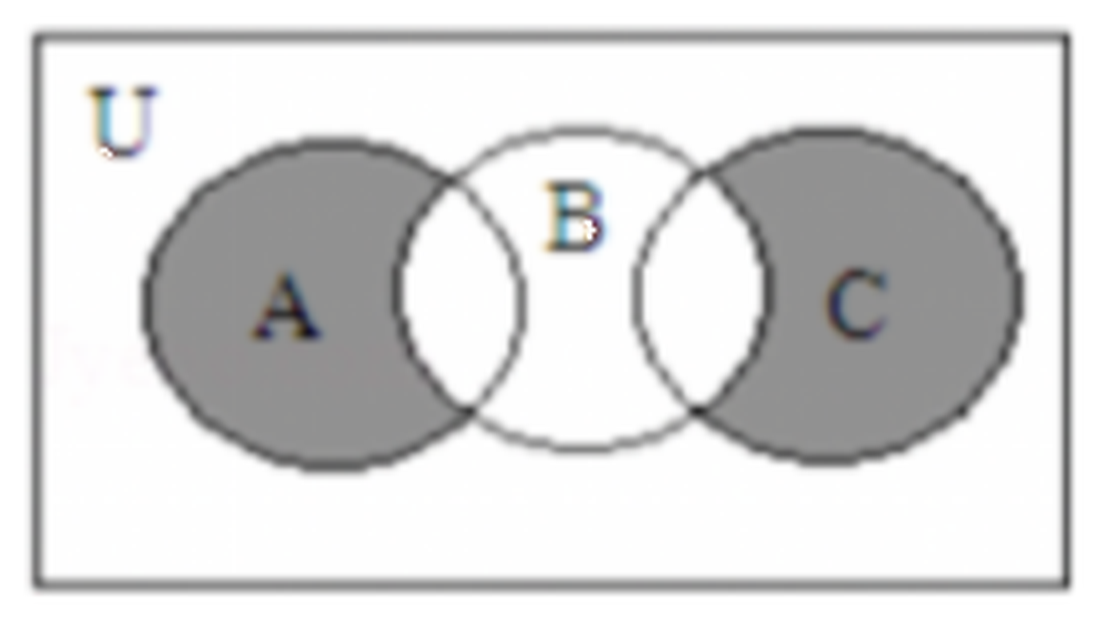
\includegraphics[width=0.40\textwidth]{figures/venn_ABC_shaded.png}
\end{center}

\ans{$(A\cup C)\cap\overline{B}$}

\item 已知集合 $A=\{1,2\}$，$B=\{-a,\,a^2+3\}$，若 $A\cup B=\{1,2,4\}$，则实数 $a$ 的值为 \blankline[2em].

\ans{$-1$}

\ifanswer
\solbegin
\step{当 $-a=4$ 时，$a=-4$，集合 $B=\{-4,19\}$，不满足 $A\cup B=\{1,2,4\}$，舍去；}
\step{当 $a^2+3=4$ 时，$a=1$ 或 $a=-1$.}
\step{当 $a=1$ 时，集合 $B=\{-1,4\}$，不满足 $A\cup B=\{1,2,4\}$，舍去；}
\step{当 $a=-1$ 时，集合 $B=\{1,4\}$，满足 $A\cup B=\{1,2,4\}$，符合题意.}
\step{综上所述，$a=-1$.}
\solend

\fi
\item 某班 45 名同学全部参加除草和植树两项劳动，依据表现评定为优秀和合格两个等级，结果如表：

\begin{center}
\begin{tabular}{|c|c|c|c|}
\hline
 & 优秀 & 合格 & 合计 \\
\hline
除草 & 30 & 15 & 45 \\
\hline
植树 & 20 & 25 & 45 \\
\hline
\end{tabular}
\end{center}

若在两个项目中都“合格”的学生最多为 10 人，则在两个项目中都优秀的同学最多为 \blankline[2em].

\ans{$15$}

\ifanswer
\solbegin
\step{设集合 $A$ 表示除草优秀的学生，集合 $B$ 表示植树优秀的学生，全班学生用集合 $U$ 表示.}
\step{则 $\overline{A}$ 表示除草合格的学生，$\overline{B}$ 表示植树合格的学生，作出 Venn 图，设两项劳动都优秀的人数为 $x$，两项劳动都合格的人数为 $y$，得 $20-x+x+30-x+y=45$，即 $x=y+5$.}
\step{因为 $y_{\max}=10$，所以 $x_{\max}=10+5=15$，即两个项目中都优秀的同学最多为 $15$.}
\solend

\fi
\item 已知集合 $M=\{x\mid 1\leqslant x\leqslant 2a-1,\,x\in\Z\}$，若集合 $M$ 有 3 个真子集，则实数 $a$ 的取值范围为 \blankline[2em].

\ans{$\left[\dfrac{3}{2},2\right)$}

\ifanswer
\solbegin
\step{由集合 $M=\{x\mid 1\leqslant x\leqslant 2a-1,\,x\in\Z\}$ 有 3 个真子集，得 $M$ 中有 2 个元素，得 $M=\{1,2\}$，所以 $2\leqslant 2a-1<3$，解得 $\tfrac{3}{2}\leqslant a<2$.}
\solend

\fi
\item 已知集合 $A=\{x\mid y=\sqrt{1-x^2},\,x\in\Z\}$，$B=\{y\mid y=x^2+1,\,x\in A\}$，则 $A\cup B=$ \blankline[2em].

\ans{$\{-1,0,1,2\}$}

\ifanswer
\solbegin
\step{$A=\{x\mid 1-x^2\geqslant 0,\,x\in\Z\}=\{-1,0,1\}$，$B=\{y\mid y=x^2+1,\,x\in A\}=\{1,2\}$，则 $A\cup B=\{-1,0,1,2\}$.}
\solend

\fi
\item 已知集合 $A=\{a,b,c,d\}$ 的所有非空真子集的元素之和为 2023，则 $a+b+c+d=$ \blankline[2em].

\ans{$289$}

\ifanswer
\solbegin
\step{因为集合 $A=\{a,b,c,d\}$ 的所有非空真子集为：$\{a\},\allowbreak\{b\},\allowbreak\{c\},\allowbreak\{d\},\allowbreak\{a,b\},\allowbreak\{a,c\},\allowbreak\{a,d\},\allowbreak\{b,c\},\allowbreak\{b,d\},\allowbreak\{c,d\},\allowbreak\{a,b,c\},\allowbreak\{a,b,d\},\allowbreak\{a,c,d\},\allowbreak\{b,c,d\}$，所以有 $7a+7b+7c+7d=2023\Rightarrow 7(a+b+c+d)=2023$ $\Rightarrow a+b+c+d=289$.}
\solend

\fi
\item 设 $S=\{r_1,r_2,\dots,r_n\}\subseteq\{1,2,3,\dots,50\}$，且 $S$ 中任意两数之和不能被 7 整除，则 $n$ 的最大值为 \blankline[2em].

\ans{$23$}

\ifanswer
\solbegin
\step{可将 $S$ 集合分为 7 组：$S_0=\{7,14,21,28,35,42,49\}$，则 $\operatorname{Card}(S_0)=7$；}
\step{$S_1=\{1,8,15,22,29,36,43,50\}$，则 $\operatorname{Card}(S_1)=8$；}
\step{$S_2=\{2,9,16,23,30,37,44\}$，则 $\operatorname{Card}(S_2)=7$；}
\step{$S_3=\{3,10,17,24,31,38,45\}$，则 $\operatorname{Card}(S_3)=7$；}
\step{$S_4=\{4,11,18,25,32,39,46\}$，则 $\operatorname{Card}(S_4)=7$；}
\step{$S_5=\{5,12,19,26,33,40,47\}$，则 $\operatorname{Card}(S_5)=7$；}
\step{$S_6=\{6,13,20,27,34,41,48\}$，则 $\operatorname{Card}(S_6)=7$.}
\step{$S$ 中的任何两个数之和不能被 7 整除，故 $S_1$ 和 $S_6$，$S_2$ 和 $S_5$，$S_3$ 和 $S_4$，$S_3$ 和 $S_5$ 不能同时取数，且 $S_0$ 中最多取一个.}
\step{所以最多的取法是取 $S_1$、$S_2$（或 $S_5$）、$S_3$（或 $S_4$）、和 $S_6$ 中的一个，故 $\operatorname{Card}(S)_{\max}=8+7+7+1=23$.}
\solend

\fi
\end{enumerate}

\bigsec{二、选择题}

\begin{enumerate}
\setcounter{enumi}{10}

\item 记 $U$ 是全集，且非空集合 $A,B$ 满足 $A\subseteq B$，则下列选项中表示空集的是（\quad）.

A. $A\cap B$\qquad B. $\overline{A}\cap B$\qquad C. $A\cap\overline{B}$\qquad D. $A\cap\overline{B}$

\ans{D}

\item 已知集合 $A=\{-1,0,1\}$，$B=\left\{(x,y)\mid x\in A,\,y\in A,\,\tfrac{x}{y}\in\mathbb{N}\right\}$，则集合 $B$ 中所含元素的个数为（\quad）.

A. $3$\qquad B. $4$\qquad C. $6$\qquad D. $9$

\ans{B}

\ifanswer
\solbegin
\step{$B=\{(-1,-1),(1,1),(0,-1),(0,1)\}$，集合 $B$ 中所含元素的个数为 4，故选 B.}
\solend

\fi

\item 已知全集为 $\mathbb{R}$，集合 $A=\{x\mid x<a\}$，集合 $B=\{x\mid x\geqslant 1\}$，若 $\overline{B}\cup A=A$，则实数 $a$ 的取值范围为（\quad）.

A. $\{a\mid a\geqslant 1\}$\qquad B. $\{a\mid a>1\}$\qquad C. $\{a\mid a\leqslant 1\}$\qquad D. $\{a\mid a<1\}$

\ans{A}

\item 设 $X$ 是一个集合，$\tau$ 是一个以 $X$ 的某些子集为元素的集合，且满足：① $X$ 属于 $\tau$，$\varnothing$ 属于 $\tau$；② $\tau$ 中任意多个元素的并集属于 $\tau$；③ $\tau$ 中有限个元素的交集属于 $\tau$，则称 $\tau$ 是集合 $X$ 上的一个拓扑. 已知集合 $X=\{a,b,c\}$，对于下面给出的四个集合 $\tau$：

①$\tau=\{\varnothing,\{a\},\{a,b\},\{a,c\}\}$；②$\tau=\{\varnothing,\{b\},\{c\},\{b,c\},\{a,b,c\}\}$；

③$\tau=\{\varnothing,\{a,c\},\{b,c\},\{c\},\{a,b,c\}\}$；④$\tau=\{\varnothing,\{a\},\{c\},\{a,b,c\}\}$.

其中是集合 $X$ 上的拓扑的集合 $\tau$ 的序号是（\quad）.

A. ②\qquad B. ①③\qquad C. ②④\qquad D. ②③

\ans{D}

\ifanswer
\solbegin
\stepm{①}{$\tau=\{\varnothing,\{a\},\{a,b\},\{a,c\}\}$：而 $\{a,b\}\cup\{a,c\}=\{a,b,c\}\notin\tau$，故①不是集合 $X$ 上的拓扑的集合 $\tau$.}
\stepm{②}{$\tau=\{\varnothing,\{b\},\{c\},\{b,c\},\{a,b,c\}\}$：满足（1）$X$ 属于 $\tau$，$\varnothing$ 属于 $\tau$；}
\stepm{（2）}{$\tau$ 中有限个元素的并集属于 $\tau$；}
\stepm{（3）}{$\tau$ 中有限个元素的交集属于 $\tau$.}
\step{因此②是集合 $X$ 上的拓扑的集合 $\tau$.}
\stepm{③}{$\tau=\{\varnothing,\{a,c\},\{b,c\},\{c\},\{a,b,c\}\}$：满足（1）$X$ 属于 $\tau$，$\varnothing$ 属于 $\tau$；}
\stepm{（2）}{$\tau$ 中有限个元素的并集属于 $\tau$；}
\stepm{（3）}{$\tau$ 中有限个元素的交集属于 $\tau$.}
\step{因此③是集合 $X$ 上的拓扑的集合 $\tau$.}
\stepm{④}{$\tau=\{\varnothing,\{a\},\{c\},\{a,b,c\}\}$：而 $\{a\}\cup\{c\}=\{a,c\}\notin\tau$，故④不是集合 $X$ 上的拓扑的集合 $\tau$.}
\step{故选 D.}
\solend

\fi
\end{enumerate}

\bigsec{三、解答题}

\begin{enumerate}
\setcounter{enumi}{14}

\item 已知集合 $U=\{x\mid 1<x\leqslant 7\}$，$A=\{x\mid 2\leqslant x<5\}$，$B=\{x\mid 3\leqslant x<7\}$，求：
\begin{enumerate}[label=(\arabic*)]
\item $\overline{A}\cap\overline{B}$；
\item $\overline{A\cap B}$.
\end{enumerate}

\ans{(1) $\{x\mid 1<x\leqslant 2\}\cup\{7\}$；（2）$\{x\mid 1<x<3\}\cup\{5\leqslant x\leqslant 7\}$}

\ifanswer
\solbegin
\stepm{(1)}{$\overline{A}=\{x\mid 1<x\leqslant 2\text{ 或 }5\leqslant x\leqslant 7\}$，$\overline{B}=\{x\mid 1<x<3\}\cup\{7\}$，因此 $\overline{A}\cap\overline{B}=\{x\mid 1<x\leqslant 2\}\cup\{7\}$；}
\stepm{（2）}{$A\cap B=\{x\mid 3\leqslant x<5\}$，所以 $\overline{A\cap B}=\{x\mid 1<x<3\text{ 或 }5\leqslant x\leqslant 7\}$.}
\solend

\fi
\ansspace[5]
\item 已知 $A=\{x\mid a\leqslant x\leqslant -a+3\}$，$B=\{x\mid x<-1\text{ 或 }x>5\}$.
\begin{enumerate}[label=(\arabic*)]
\item 若 $A\cap B=\varnothing$，求实数 $a$ 的取值范围；
\item 若 $A\cup B=\R$，求实数 $a$ 的取值范围.
\end{enumerate}

\ans{(1) $a\geqslant -1$；（2）$a\leqslant -2$}

\ansspace[5]
\item 已知集合 $A=\{a^2,a+2,2\}$.
\begin{enumerate}[label=(\arabic*)]
\item 若 $-1\in A$，求实数 $a$ 的值；
\item 若 $B=\{-2,2\}$，且 $A\cap B$ 的元素个数为 2，求实数 $a$ 的值；
\item 若 $4\in A$，求实数 $a$ 的值.
\end{enumerate}

\ans{(1) $-3$；（2）$-4$；（3）$-2$}

\ifanswer
\solbegin
\stepm{(1)}{由题意得 $a+2=-1$，解得 $a=-3$，此时 $A=\{9,-1,2\}$，所以实数 $a$ 的值为 $-3$；}
\stepm{(2)}{因为 $B=\{-2,2\}$，且 $A\cap B$ 的元素个数为 2，所以 $a+2=-2$，解得 $a=-4$，此时集合 $A=\{16,-2,2\}$，$A\cap B=\{-2,2\}$，所以实数 $a$ 的值为 $-4$；}
\stepm{(3)}{由题意得 $a^2=4$ 或 $a+2=4$，则 $a=\pm 2$.}
\step{当 $a=2$ 时，$A=\{4,4,2\}$，不成立，舍去；}
\step{当 $a=-2$ 时，$A=\{4,0,2\}$，所以实数 $a$ 的值为 $-2$.}
\solend

\fi
\ansspace[7]
\ansneed{7cm}
\item 设数集 $A$ 由实数构成，且满足：若 $x\in A(x\neq 1\text{ 且 }x\neq 0)$，则 $\dfrac{1}{1-x}\in A$.
\begin{enumerate}[label=(\arabic*)]
\item 若 $2\in A$，试证明 $A$ 中还有另外两个元素；
\item 集合 $A$ 是否为双元素集合，并说明理由；
\item 若 $A$ 中元素个数不超过 8 个，所有元素的和为 $\tfrac{14}{3}$，且 $A$ 中有一个元素的平方等于所有元素的积，求集合 $A$.
\end{enumerate}

\ans{(1) 略；（2）否；（3）$\left\{-1,\dfrac{1}{2},2,-\dfrac{1}{2},3,\dfrac{2}{3}\right\}$}

\ifanswer
\solbegin
\stepm{(1)}{因为 $2\in A$，所以 $\tfrac{1}{1-2}=-1\in A$，所以 $\tfrac{1}{1-(-1)}=\tfrac{1}{2}\in A$，所以集合 $A$ 中还有另外两个元素 $-1$ 和 $\tfrac{1}{2}$；}
\stepm{(2)}{若 $x\in A(x\neq 1,x\neq 0)$，则 $\tfrac{1}{1-x}\in A$，则 $\tfrac{1}{1-\tfrac{1}{1-x}}=1-\tfrac{1}{x}\in A$.}
\step{若 $1-\tfrac{1}{x}\in A$，则 $x\in A$，所以集合 $A$ 中应包含 $x$、$\tfrac{1}{1-x}$、$1-\tfrac{1}{x}$.}
\step{检验得 $x$、$\tfrac{1}{1-x}$、$1-\tfrac{1}{x}$ 互不相等，所以集合 $A$ 不是双元素集合；}
\stepm{(3)}{由 (2) 得集合 $A$ 中的元素个数应为 3 或 6.}
\step{因为 $x\left(\tfrac{1}{1-x}\right)\left(1-\tfrac{1}{x}\right)=-1$，且 $A$ 中有一个元素的平方等于所有元素的积，所以 $A$ 中应有 6 个元素，且其中一个元素为 $-1$.}
\step{因为 $-1\in A$，结合条件得 $-\tfrac{1}{2}\in A$，$2\in A$.}
\step{因为 $-1+\tfrac{1}{2}+2=\tfrac{3}{2}$，所以剩余的三个元素和为 $\tfrac{19}{6}$，即 $x-\tfrac{1}{x}+\tfrac{x-1}{x}=\tfrac{19}{6}$，解得 $x=-\tfrac{1}{2},3,\tfrac{2}{3}$.}
\step{所以 $A=\left\{-1,\tfrac{1}{2},2,-\tfrac{1}{2},3,\tfrac{2}{3}\right\}$.}
\solend

\fi
\ansspace*[10]
\end{enumerate}

\end{document}